\documentclass[a4paper,twoside]{article}
\usepackage{autiwa}
\title{Astuces Inkscape\\version 1.2}
\author{Autiwa}
\makeindex
\begin{document}
\begin{titlepage}
\begin{center}
~
\vfill
% Upper part of the page
\begin{figure}[t]
\centering
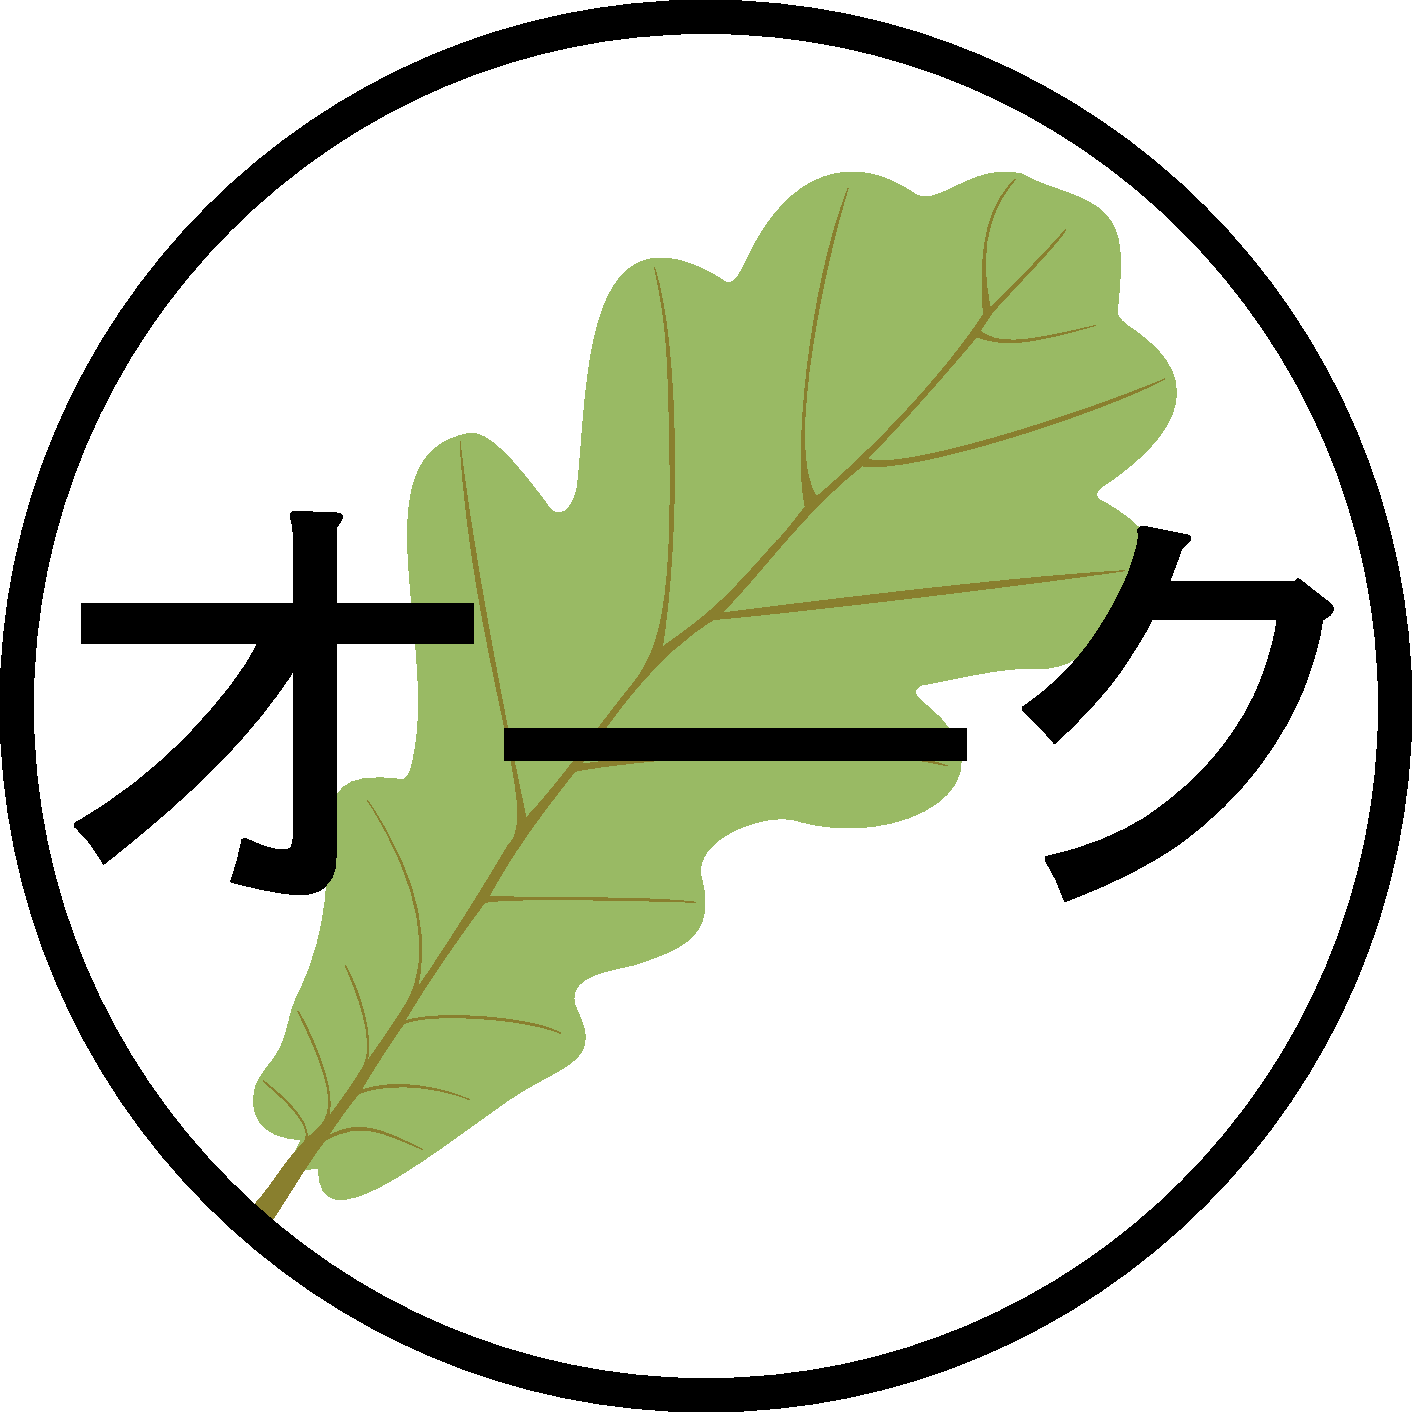
\includegraphics[width=0.15\textwidth]{logo-autiwa.pdf}%chemin absolu de l'image pour que l'on puisse appeler ce fichier depuis plusieurs dossiers différents.
\end{figure}

% Title
\HRule \\[0.4cm]
{ \huge \bfseries \makeatletter\@title\makeatother}\\[0.4cm]

\HRule \\[0.75cm]
{\large \today}\\[0.75cm]
\makeatletter
\@author
\makeatother
\vfill
\vfill
~
% Bottom of the page


\end{center}
\end{titlepage}

\tableofcontents
\newpage

% \section{Indices et exposants (subscript, superscript)}
% À première vue, il n'y a rien dans Inkscape qui permet de faire cela. Il existe un moyen un peu détourner de le réaliser cependant. Il suffit d'écrire normalement, puis de sélectionner la partie que l'on souhaite mettre en indice ou en exposant. Ensuite, à l'aide de \touche{Alt}+\touche{\textuparrow} et \touche{Alt}+\touche{\textdownarrow}, on peut mettre en indice ou exposant en appuyant plusieurs fois (pour ma part, je mets une police plus petite de 4 points, et je descend ou monte de 7 ou 8 \og coups\fg (comprendre que je fais 7 fois le raccourci précédemment évoqué).

\section[LaTeX avec Inkscape]{\LaTeX avec Inkscape}
Pour avoir l'option Effet>Rendu>Formule LaTeX... il faut installer \gras[logiciel!pstoedit]{pstoedit} en plus d'inkscape. L'option apparaît automatique au démarrage suivant.

\section{Général}
\subsection{Sélection à l'aide du dialogue Rechercher}
Un moyen très pratique pour sélectionner des objets est d'utiliser la fonction \og Rechercher\fg (\touche{Ctrl}+\touche{F}). En effet, une des fonctions très utile est de pouvoir sélectionner les objets par type. Ainsi, sélectionner tous les chemins, ou tous les textes, en un seul coup, sans devoir tout sélectionner à la main.

D'autres champs sont disponibles qui parlent d'eux mêmes et permettent d'affiner les recherches.

\subsection{Sélection à la souris}
Cette section couvre la sélection d'objets à la souris. En ajoutant \touche{Ctrl} à de nombreuses commandes ci-dessous. 

\touche{Clic gauche} de la souris : sélectionner un objet. Sélectionne un objet en cliquant dessus.

\touche{Maj}+\touche{Clic gauche} de la souris : alterner la sélection. Ajoute ou soustrait un objet d'une sélection . Ceci permet la sélection d'objets multiples. Si l'objet cliqué n'est pas déjà sélectionné, il le sera. S'il est déjà sélectionné, il sera désélectionné.

\touche{Alt}+\touche{Clic gauche} de la souris : sélectionner dessous. Sélectionne l'objet suivant sous l'objet de la sélection courante sous le pointeur. Ceci permet de sélectionner des objets recouverts par d'autres. Répétez cette manipulation pour descendre dans l'Ordre-z. Si l'objet le plus bas est déjà sélectionné, cette manipulation sélectionnera l'objet le plus haut.

Tirer avec le Bouton gauche de la souris : sélectionner de multiples objets. Lorsqu'on démarre d'un espace vide, cette manipulation sélectionne tous les objets compris entièrement à l'intérieur du rectangle formé entre le point de départ et le point d'arrêt de l'étirement. C'est ce qu'on appelle généralement une sélection par Étirement. La zone de sélection correspond à la ligne dessinée temporairement pendant l'étirement.

Tirer avec \touche{Maj}+Bouton gauche de la souris : ajouter des objets à une sélection multiple. Ajoute des objets à une sélection par étirement pré-existante. Empêche de plus la sélection d'un objet situé sous le point de départ de l'étirement (sans la touche \touche{Maj}, un objet situé sous le point de départ de l'étirement est sélectionné et déplacé). Les objets précédemment sélectionnés par étirement ne sont pas désélectionnés.

Tirer avec \touche{Alt}+Bouton gauche de la souris : sélectionner des objets multiples par contact. Ceci sélectionne tous les objets touchés par le curseur de la souris pendant l'étirement. Une ligne rouge indique le chemin emprunté par le curseur. Ceci est très utile lorsqu'on a besoin de sélectionner de multiples chemins comme on en trouve dans des gravures ou des cheveux. Le maintient de la touche \touche{Maj} enfoncée empêche la sélection d'un objet déjà sélectionné si l'étirement commence au-dessus de cet objet.
Sélection par contact.
Tirer avec \touche{Alt}+Bouton gauche de la souris pour « toucher » sélectionne les chemins un à un.

Tirer avec \touche{Maj}+\touche{Alt}+Bouton gauche de la souris : ajouter à une sélection des objets multiples par contact. Ceci ajoute les objets touchés à la sélection. Elle peut également être utilisée lorsque l'étirement commence sur un objet déjà sélectionné. 

Les objets à l'intérieur d'un Groupe peuvent être sélectionnés, voir \refsec{sec:groupes}

\section{Motifs}
\subsection{Espacer des motifs}
Généralement, les motifs n'ont pas d'espaces entre leurs répétitions. Qu'à celà ne tienne, il suffit de définir l'espace à même le motif. Par exemple, au lieu de faire un cercle tout bête. Faites en un petit, qui sera la taille nominale du cercle, puis un plus grand qui déterminera l'espace autour dudit cercle. Le cercle le plus grand, dupliquez le (\touche{Ctrl}+D), puis fusionnez les trois chemins en un seul (\touche{Ctrl}+K après les avoir sélectionnés tout les trois). Ensuite, vous remplissez le motif, en sélectionnant qu'un chevauchement rend la somme transparente (et trois sera de nouveau opaque), puis vous enlevez le contour (couleur transparente), et vous avez votre espace.

\begin{remarque}
C'est une technique que j'ai utilisée pour \og motif suivant un chemin\fg, et ainsi pouvoir définir un espace entre les cercles, mais ça doit être utile pour autre chose je pense. Ce que je n'avais pas compris de suite, c'est qu'une fois le chemin rempli des motifs, modifier le contour ou le remplissage du chemin agissait directement sur le contour et le remplissage des motifs, ce qui change tout.
\end{remarque}

\section{Clones}
\subsection{Sélectionner l'original}
Pour sélectionner l'original d'une série de clones rapidement, il suffit de sélectionner un clone, et de faire \touche{Maj}+D.

\section{Chemins}
\subsection{Flèches dans le bon sens}
Il m'arrivait souvent d'avoir des flèches dans le mauvais sens. C'est à dire qu'en définissant une flèche au n\oe ud final, la flèche n'était pas à l'endroit voulu. Il est possible d'inverser le sens d'un chemin (basiquement, inverser le n\oe ud de départ et le n\oe ud d'arrivé, sans que ça ne change rien à la forme du chemin) via le menu Chemin>Inverser.

\subsection{Éroder et Dilater}
Inkscape peut étendre et contracter des objets par une modification de leurs dimensions, mais aussi par offset du chemin, c'est-à-dire par un déplacement perpendiculaire en tout point du chemin. Les commandes correspondantes sont Éroder (\touche{Ctrl}+\touche{(}) et Dilater (\touche{Ctrl}+\touche{)}).

Les commandes éroder et dilater produisent des chemins (si nécessaire en convertissant l'objet original en chemin). Un offset dynamique (\touche{Ctrl}+\touche{J}) sera souvent plus pratique : il crée un objet avec une poignée déplaçable qui contrôle le rayon d'offset.

Un tel objet offset dynamique retient le chemin d'origine, et ainsi ne se \og dégrade\fg pas quand vous modifiez un grand nombre de fois la distance d'offset. Quand vous n'avez plus besoin de l'ajuster, vous pouvez toujours le convertir de nouveau en chemin.

Encore plus pratique : l'offset lié (\touche{Ctrl}+\touche{Alt}+\touche{J}), similaire à un offset dynamique mais connecté au chemin qui reste éditable. Vous pouvez en créer autant que vous voulez à partir d'un chemin source. En éditant les n\oe uds du chemin original, celà modifiera automatiquement les offset liés. Vous pouvez aussi redimensionner ou appliquer une rotation au chemin original, ça sera automatiquement appliqué à l'offset lié. En déplaçant l'offset lié, vous pouvez ainsi faire une ombre portée, et un déplacement du chemin original déplacera automatiquement l'offset lié pour que leurs positions relatives ne changent pas.

\subsection{Effets de chemin}
Ces trois paragraphes d'explications ont étés pris sur le site \\
\url{http://www.pixenjoy.com/inkscape-046-live-path-effects}
\subsubsection{Courber un chemin}

Cet effet permet de courber un chemin le long d'un autre chemin. Lorsque l'effet \og Courber un chemin\fg  est appliqué à un chemin A, ce chemin peut être courbé le long d'un autre chemin B (que l'on appellera \og chemin courbé\fg ). Avec l'éditeur de n\oe uds, le chemin A et le chemin courbé B peuvent être modifié sur le canevas et le résultat se met à jour instantanément.

Dans la fenêtre de dialogue des \og Effets de chemin\fg  (\touche{Maj}+\touche{Ctrl}+7), après avoir cliqué sur le bouton \og Appliquer\fg , vous trouverez à côté du libellé \og Chemin de courbure\fg  trois boutons. Un bouton vous permettant d'éditer sur le canevas le chemin courbé (Editer sur la zone de travail), un bouton vous permettant de coller un nouveau chemin courbé enregistré dans le presse papier et un bouton vous permettant de le coller.

Cas pratique :
\begin{enumerate}
\item Tracer votre chemin B qui servira de modèle et le long duquel viendra se déformer le chemin A.
\begin{exemple}
Prenez par exemple un rectangle pour le chemin A, et pour le chemin B deux points reliés par une courbe simple que vous aurez tout le loisir de faire varier par la suite.
\end{exemple}
\item Sélectionnez et copier dans le presse-papier le chemin B.
\item Sélectionnez le chemin A que vous voulez déformer. Il doit bien s'agir d'un chemin et non d'un groupe de forme ou d'une forme. Transformez vos formes en un chemin unique pour pouvoir appliquer les \og effets de chemins\fg . Pour cela, si vous travaillez sur une seule forme, sélectionnez la puis : Chemin > Objet en chemin. Si vous avez un groupement de formes, dégroupez les (Objet > Dégrouper), sélectionnez-les tous puis unifiez-les : Chemin > Union.
\item Ouvrez la boite de dialogue des effets de chemin : (\touche{Maj}+\touche{Ctrl}+7) ou Chemin > Effets de chemin
\item Appliquer l'effet \og Courber un chemin\fg
\item Collez le chemin courbé en cliquant sur le bouton (représenté par une icône) \og Coller le chemin\fg  qui se trouve à côté du libellé \og Chemin de courbure\fg
\item Pour éditer les chemins, cliquez sur le bouton (représenté par une icône) \og Editer sur la zone de travail\fg
\end{enumerate}



\subsubsection{Motif suivant un chemin}
Cet effet permet de courber un chemin le long d'un autre chemin. Quand cet effet est appliqué à un chemin A (appelé squelette) un autre chemin B (appelé motif) peut être passé en paramètre. Le résultat est que le chemin B est courbé le long du chemin A. Avec l'outil d'édition des n\oe uds, le chemin peut être modifié sur l'espace de travail et le résultat est mis à jour en temps réel.

Vous pouvez choisir le motif pour le squelette sélectionné en le collant dans l'espace de travail à partir du presse-papier (c'est-à-dire que vous sélectionnez et vous copiez dans le presse-papier le motif (ou le chemin), ensuite vous sélectionnez le squelette, vous appliquez l'effet \og Motif suivant un chemin\fg, et vous cliquez sur \og collez le motif\fg). Dans la fenêtre de dialogue des \og Effets de chemin\fg  (\touche{Ctrl}+\touche{Shift}+7), le paramètre \og Largeur\fg  vous permet de changer la largeur du motif appliqué au chemin.

Cas pratique :
\begin{enumerate}
\item Choisissez un motif (chemin B) qui viendra se positionner sur un squelette (chemin A). N'oubliez pas de le transformer en un chemin unique si ce n'est pas déjà le cas.
\item Sélectionnez et copiez le motif, chemin B, dans le presse-papier.
\item Dessinez le squelette, chemin A, sur lequel le motif viendra se positionner et sélectionnez le.
\item Ouvrez la boite de dialogue des effets de chemin : (\touche{Maj}+\touche{Ctrl}+7) ou Chemin > Effets de chemin
\item Appliquer l'effet \og Motif suivant un chemin\fg
\item Vous pouvez choisir de répéter ou pas le motif en sélectionnant une des options proposée dans le menu déroulant \og Copies du motif\fg
\item Collez le motif en cliquant sur le bouton (représenté par une icône) \og Coller le chemin\fg  qui se trouve à côté du libellé \og Chemin de courbure\fg
\item Vous pouvez éditer le motif pour modifier sa forme, cliquez sur le bouton (représenté par une icône) \og Editer sur la zone de travail\fg
\end{enumerate}

\subsubsection{Relier les sous-chemins}


L'effet \og Relier les sous-chemins\fg  relie les points de deux sous-chemins d'un chemin avec des lignes droites ou des segments courbés. Le résultat obtenu ressemble à du \og String Art\fg.

La forme des chemins connectés peut être contrôlé par le paramètre \og Editer sur la zone de travail\fg . Ce procédé peut être utilisé pour dessiner une chevelure en reliant les chemins au niveau de la pointe. D'autres contrôles concernent le nombre de chemins, la variation de l'espace entre les chemins connectés (faisceau) et aussi si le début et la fin des pointes de la maille doit être exactement sur la sous-courbe d'origine ou peut dévier aléatoirement autour d'elle. Enfin la largeur des traits peut être modifié.

Notez que cet effet ne peut être appliqué uniquement que sur un chemin composé de deux sous-chemins. Utilisez Chemin > Combiner (\touche{Ctrl} + K) pour créer un tel chemin à partir de deux chemins séparés.

Cas pratique :
\begin{enumerate}
\item Tracer deux chemins A et B.
\item Combinez les deux chemins pour ne former qu'un seul chemin : sélectionnez A et B et cliquez sur \touche{Ctrl}+K.
\begin{exemple}
ça marche bien avec deux lignes, l'une horizontale, et l'autre vecticale.
\end{exemple}
\item Sélectionnez la combinaison obtenu.
\item Ouvrez la boite de dialogue des effets de chemin : (\touche{Maj}+\touche{Ctrl}+7) ou Chemin > Effets de chemin
\item Appliquez l'effet \og Relier les sous-chemins\fg
\item Dans la partie \og Effet courant\fg , vous disposez d'un contrôle sur plusieurs paramètres pour transformer votre maillage : nombre de chemins \dots
\item En cliquant sur l'icône \og Editer sur la zone de travail\fg , vous éditez un chemin sur la zone de travail qui vous permet de modifier l'orientation du maillage.
\end{enumerate}

\section{Groupes}\label{sec:groupes}
\subsection{Sélection dans un groupe}
Les objets des Groupes peuvent être édités et manipulés sans séparer le Groupe. Les commandes suivantes sélectionnent les objets à l'intérieur des Groupes :

\touche{Ctrl}+Clic gauche de la souris : sélectionner à l'intérieur d'un groupe. Sélectionne un objet à l'intérieur d'un Groupe. Cette commande sélectionne les objets indépendamment du nombre de niveaux de Groupes auxquels ils sont intégrés.

\touche{Ctrl}+\touche{Alt}+Clic gauche de la souris : sélectionner dessous à l'intérieur d'un groupe. Sélectionne un objet au sein d'un Groupe situé sous le curseur et juste en dessous, dans l'Ordre-z, de l'objet de la sélection courante. Si l'objet de la sélection courante est situé tout en bas dans l'Ordre-z, l'objet du haut est sélectionné. Cette commande sélectionne les objets indépendamment du nombre de niveaux de Groupes auxquels ils sont intégrés.

\touche{Maj}+\touche{Ctrl}+\touche{Alt}+\touche{Clic gauche} de la souris : alterner à l'intérieur d'un groupe. Ajoute à une sélection un objet non sélectionné ou supprime d'une sélection un objet sélectionné appartenant à un Groupe. 

On peut entrer dans un Groupe ou le transformer en Calque temporaire pour l'édition. Deux façons d'entrer dans un groupe et de sortir d'un groupe sont disponibles :

\touche{Ctrl}+\touche{Entrée} à partir d'un Groupe sélectionné pour y entrer. Répétez cette manipulation pour entrer dans un groupe de niveau inférieur (sous-groupe). \touche{Ctrl}+\touche{Retour} pour sortir du Groupe. Vous sortez d'un niveau de groupe.

\begin{remarque}
Pour ajouter un objet existant à un Groupe existant, coupez l'objet (Édition → icône Couper (\touche{Ctrl}+\touche{X})), entrez dans le Groupe (Double-clic gauche de la souris) puis collez-le sur place (Édition → icône Coller sur place (\touche{Ctrl}+\touche{Alt}+\touche{V})). 
\end{remarque}




\section{Textes}
\subsection{Encadrer ou mettre en forme un texte}
On peut mettre un texte dans un cadre, ce qui permet des choses assez poussées. On peut par exemple répartir le texte dans plusieurs formes. 

\begin{attention}
Il faut définir le texte en faisant un glisser déposer pour y définir un cadre, il ne faut pas se contenter de définir un texte en cliquant dans un calque. C'est à dire qu'une fois l'outil texte activé, il faut faire un clic gauche, rester appuyé sur le clic gauche, définir un cadre en relachant le clic à l'endroit voulu pour le coin en bas à droite du cadre. 
\end{attention}

Une fois le texte défini, définissez vos formes, soit une seule, soit plusieurs. Une fois fait, sélectionnez le texte, puis, sélectionnez les formes dans l'ordre inverse de l'ordre dans lequel vous voulez que le texte les remplisse. C'est à dire que si vous avez trois formes A, B et C, que vous voulez que le texte remplisse A, puis B puis C, vous devez sélectionner le texte, puis la forme C, puis la forme B puis la forme A.

Une fois les 4 objets sélectionnés, activez l'option Texte>Encadrer.


\section{Masques d'objets}
Disponible via Objet>Masque>Définir. Cette fonction permet de \og découper\fg un ou plusieurs chemins. En effet, si on sélectionne plusieurs chemins, le masque sera défini à partir du chemin le plus au-dessus (avec le z le plus élevé), et s'appliquera à tout les autres chemins sélectionnés. Les caractéristiques du chemin le plus au-dessus sont importantes, c'est à dire la couleur de remplissage, son opacité et cie. Ceci seront autant de caractéristiques qui s'appliqueront en tant que masque aux autres chemins. En clair, pour simplement tronquer ce qui va apparaître à l'écran, sans rien modifier d'autre, on fera attention à ce que le chemin du dessus aie un remplissage blanc, opacité maximale et sans contour. C'est un procédé non destructif, c'est à dire qu'on peut retirer le masque par la suite et récupérer les chemins tels qu'ils étaient avant.

Voici à quoi celà peut servir concrêtement : celà permet de tronquer les flous. Vous avez surement remarqué qu'en mettant un flou de 4\%, la couleur dépassait un peu de la taille de chemin initiale. Il peut arriver que l'on veuille que la couleur s'arrête exactement aux bords, y compris le flou. Pour celà, on duplique le chemin, et le chemin dupliqué, mis blanc, est ensuite appliqué en tant que masque par la méthode expliquée ci-dessus.

Essayez par exemple de faire ça avec un cercle tout bête, sans remplissage, mais simplement avec un contour, que vous floutez à 5\%. Dupliquez ensuite ce même cercle, enlevez le contour, mettez un remplissage blanc opaque, sélectionnez le cercle normal et le cercle blanc (le cercle blanc doit être au dessus du cercle normal), puis appliquez le masque. Vous pouvez maintenant supprimer le cercle blanc et regarder le résultat obtenu.

\begin{remarque}
Pour l'exemple du cercle, il sert juste à montrer ce que ça donne, de manière simple. En effet, il est tout à fait possible d'obtenir le même résultat avec un dégradé radial approprié, ce qui rend la méthode du masque inutile dans ce cas là. Pour d'autres cas par contre, l'emploi du masque se révèlera irremplaçable.
\end{remarque}







\section{Système de Lindenmayer}
Ceci permet de réaliser des fractales relativement complexes. En guise d'exemple, je vais expliquer comment faire un flocon de neige à partir d'une étoile avec cet effet.

\begin{tabular}{>{\bfseries}r<{}@{ : }p{11cm}}
caractère &	Effet dans la règle\\
A, B, C, D, E, F & dessine un trait vers l'avant de la longueur déterminée par la \textbf{longueur d'incrément}\\
G, H, I, J, K, L & déplace vers l'avant de la longueur déterminée par la \textbf{longueur d'incrément}\\
+ &	Effectue une rotation vers la droite de l'angle déterminée par \textbf{angle droit}\\
- &	Effectue une rotation vers la droite de l'angle déterminée par \textbf{rotation à gauche}\\
| &	Effectue une rotation de 180\degre\\
\verb|[| &	Mémorise le point actuel\\
\verb|]| &	se rend au point mémorisé précédemment
\end{tabular}

Déjà, autant le préciser de suite, je ne sais pas à quoi sert la partie \og Axiome\fg. Je ne sais pas non plus pourquoi il y a plusieurs lettres pour symboliser les traits. L'ordre détermine le nombre d'itération que l'on va effectuer. Concrêtement, chaque itération remplace les segments de l'itération précédente par la ou les règles que l'on a donné (quand il y a plusieurs règles, je sais pas comment ça marche)

\begin{remarque}
Après avoir essayé sur un segment simple et avoir trituré l'axiome, il semble que l'axiome représente la forme de base que l'on va ensuite modifier. C'est à dire qu'avec \texttt{F++F++F}, ça signifie que la forme de base sera un triangle équilatéral. J'ai même pu faire un flocon de neige sans sélectionner de chemin à la base, donc je me demande si c'est très utile de sélectionner un chemin.

En conséquence, les différentes lettres permettraient de particulariser différents types de segments.
\end{remarque}

Je ne vais pas recopier les différents styles que j'ai pu rencontrer, voici le lien où j'ai trouvé ce que j'ai pu apprendre :
\url{http://inkscape.osuosl.org/screenshots/gallery/inkscape-0.44-lindenmayer.png}

\subsection{Flocon de Neige}
\begin{tabular}{>{\bfseries}r<{}@{ : }p{6cm}}
option &	valeur\\
Axiome & F++F++F\\
Règles & F=F-F++F-F\\
Ordre & 5\\
Longueur d'incrément (px) & 5,0\\
Rendre les incréments aléatoires (\%) & 0,0\\
Rotation à gauche & 60\\
Angle droit & 60 \\
Rendre l'angle aléatoire & 0
\end{tabular}

\begin{remarque}
Vous remarquerez que la règle donnée pour les flocons de neige s'explicite relativement bien. Il est facile de voir que pour chaque segment, elle va faire un trait, puis tourner de 60 degrés vers la gauche, autre trait, puis tourner de 60 degrés vers la droit par rapport à la direction initiale (c'est à dire 120\degre vers la droite depuis le segment précédent), puis nouveau trait, et enfin, on trace un trait dans la même direction que la direction initiale, c'est à dire qu'on retourne de 60\degre vers la gauche. (une sorte de chapeau quoi.

Pour visualiser très simplement ce que fait la règle, faire un essai à l'ordre 1 sur un segment simple, et vous verrez la forme de la règle.
\end{remarque}



\printindex
\end{document}